\documentclass[A4paper, 12pt]{article}
\usepackage{fancyhdr}
\usepackage{graphicx}
\usepackage{booktabs}
\usepackage{pdfpages}
\usepackage{ragged2e}
\usepackage[utf8]{inputenc} % this is needed for umlauts
\usepackage[ngerman]{babel} % this is needed for umlauts
\usepackage[T1]{fontenc}    % this is needed for correct output of umlauts in pdf
\setlength{\RaggedRightParindent}{\parindent}
\pagestyle{fancy}
\lhead{Vulcano 2.0: Ein Neuer Anfang}
\rhead{v2.03}
\cfoot{\thepage}
\renewcommand{\headrulewidth}{0.4pt}
\renewcommand{\footrulewidth}{0.4pt}
\begin{document}
\RaggedRight
\title{Vulcano 2.0: Ein Neuer Anfang}
\author{The Vulcano Team}
\date{\today}
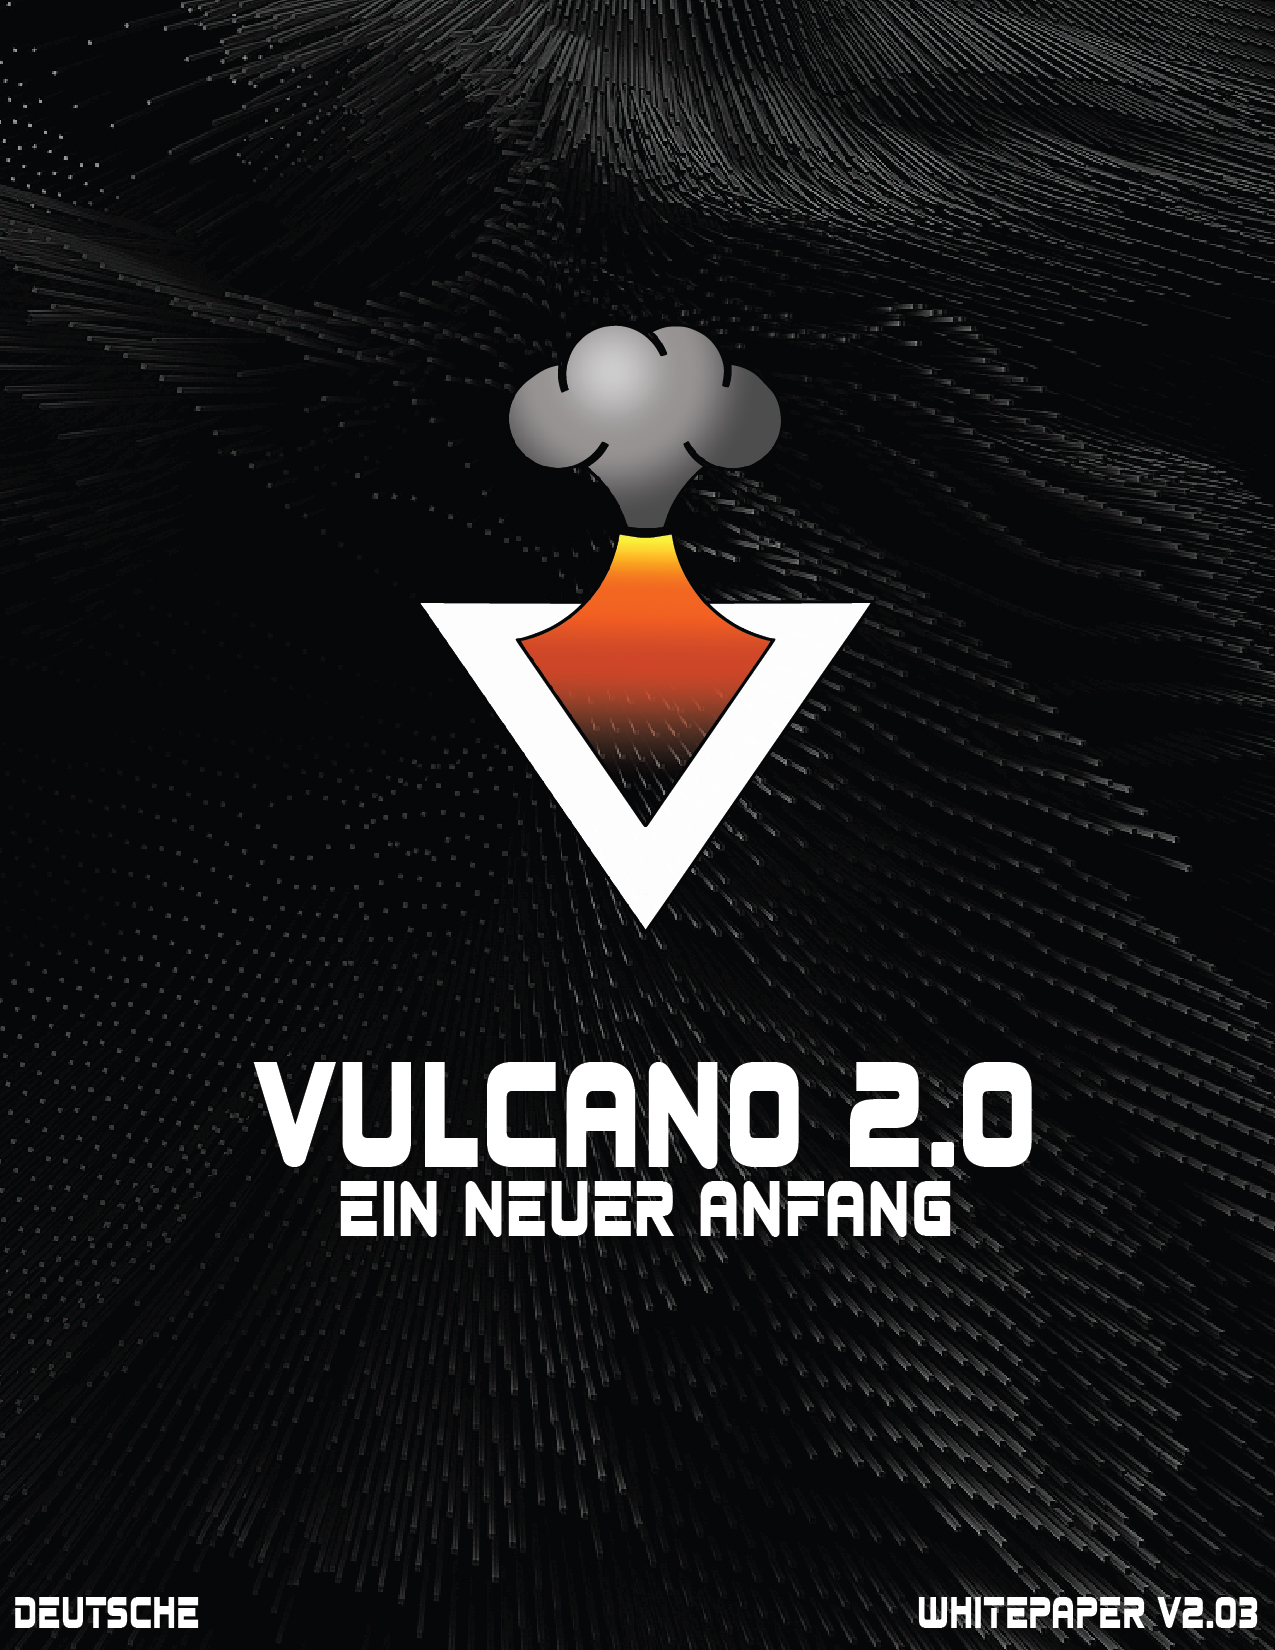
\includepdf[pages=1]{COVER-GER.jpg}
\newpage
\tableofcontents
\newpage
\section{Einleitung}

Vulcano (Bezeichnung: VULC) ist eine gemeinschaftsorientierte Münze, die ursprünglich Ende 2017 von einem nun komplett abwesenden Entwicklerteam entwickelt wurde. Anfänglich war es nur ein "High Staking Coin" mit einer jährlichen Rendite von 950\%. Aufgrund mehrerer Fehler seitens des ursprünglichen Entwicklungs Teams lag die tatsächliche Rate näher an 320,000\%. Dies ist unbemerkt geblieben, bis ein Mitglied der Gemeinschaft dies durch die Untersuchung der Blockchain aus dem Genesis Block 1 berechnete. Sobald diese grundlegende Schwäche offengelegt war, kam das neue Vulcano-Team, bestehend aus Mitgliedern der Gemeinschaft, zusammen, um das Vulcano-Projekt sowohl auf technischer als auch auf philosophischer Ebene durch einen vollständigen Wiederaufbau und die Entwicklung eines realen Anwendungsfalls zu retten. In diesem Whitepaper wird eine Strategie für ein vollständiges Upgrade von Vulcano dargelegt und ein Neustart der neu aufgerüsteten Münze als Mittel zur Finanzierung von Exploration und Forschung der Geothermie. 

Anstatt einfach das Prozentsatz-Problem von Vulcano zu lösen, haben wir beschlossen, die Münze komplett auf einer neuen Codebasis zu aktualisieren. Um den Vulcano Core am besten zu modernisieren, hat das Vulcano Team auf Bulwark als Code-Basis entschieden. Bulwark baut auf PIVX auf, das selbst auf der beliebten DASH-Kryptowährung basiert. Diese kritische Entscheidung gibt uns die Möglichkeit, Masternode-Funktionalitäten, Governance und schließlich die Integration von Hardware-Nodes zur Unterstützung des Vulcano Ökosystems zu vewenden. Damit schaffen wir ein wahrhaft dezentralisiertes System von Governance und Coin-Staking und Netzwerksicherheit. Dieses Dokument wird auch die zukünftigen Pläne für die Legitimation von Vulcano darstellen durch die Gründung der Vulcano Foundation, ein geplantes  Nonprofit-Unternehmen mit Sitz in den USA, das Vulcano in einer ausgereiften Art und Weise wachsen lässt und dabei hilft, sich mit dem Rest der Geschäftswelt zu verbinden und integrieren, und anfängt, sich in Verhandlungen zu involvieren. Dies ist besonders wichtig, da der langfristige Anwendungsfall von Vulcano den Erwerb eines Portfolios von geistigem Eigentum durch den nachstehend erläuterten Forschungsmechanismus erfordert. Durch die Schaffung eines Portfolios von geistigem Eigentum für die Finanzierung von Forschung an Universitäten und Forschungseinrichtungen auf der ganzen Welt würde die Vulcano Foundation es uns ermöglichen, dieses geistige Eigentum bestmöglich zu nutzen. 
Dies ist ein absolut kritischer Schritt, der dem dezentralen Vulcano erlauben wird, mit Projekten der zentralen Welten des Geschäfts und der Wissenschaft zu interagieren und sich zu verbinden. 

In diesem Dokument werden auch die geplanten Prozentsätze der Governance-Gebühren dargelegt, welche direkt zur Finanzierung der geothermischen Forschung verwendet werden, um sowohl die Wissenschaft voranzubringen als auch geistiges Eigentum zu gewinnen, um der Vulcano Foundation mehr Finanzierung für zukünftige Entwicklungen und zur Finanzierung von zusätzlichen Zuschüssen einzubringen. 

Was Sie in diesem Dokument nicht finden werden, sind wilde und unbegründete Versprechungen über die Zukunft der Vulcano Blockchain. Vulcano strebt nach Innovation und Wachstum, ohne Versprechen zu machen, die nicht eingehalten werden können. Stattdessen widmen wir unsere Ressourcen der Forschung und dem technologischen Fortschritt. Alle Blockchain-Technologien, die in diesem Dokument erwähnt werden, wurden bereits demonstriert und können zu gegebener Zeit aktiviert werden. Wir glauben, dass es an der Zeit für die Kryptowährungs-Gemeinschaften ist, so zu handeln, wie es im Einklang mit dem Geschäftspotenzial ist, das sie an den Tisch bringen, und dass wilde Behauptungen über die Blockchain-Technologie nicht benötigt werden, um ein Geschäftsszenario für die Nutzung bestehender Technologien zu erstellen. Entwickler, Teamleiter und die Gesellschaften selbst müssen verstehen, dass, wenn man vom größeren Umfeld, Unternehmen und akademischen Gemeinschaften akzeptiert werden will, man bereit sein muss, bis zu einem gewissen Grad nach ihren Regeln zu spielen und Gebrauch von dem zu machen, was man hat, bevor man voranschreitenden Ideen über unbewiesene Blockchain-Technologien – bevor sie geplant, entwickelt oder getestet wurden – den Weg bereiten kann. Zwar könnte es in der Zukunft Fortschritte in der Blockchain-Technologie für Vulcano selbst geben, jedoch wird seine Veröffentlichung nicht mit Monaten an lautem Getöse und Marketing kommen, es wird nur darüber gesprochen werden, sobald es bereits fertig ist und bereits entwickelt wurde. Wir glauben, dass diese Methode der bedeckten Entwicklung am besten für die Währung ist, weil es spekulative Investitionen begrenzt und den Aufbau einer stabilen Grundlage für die Plattform in der Zukunft erlaubt. 

Unser Ziel ist es, Vulcano zu einer der wichtigsten Finanzierungsquellen für die Nachhaltigkeitsforschung in der Zukunft zu machen und um schließlich ein Geschäft im Ökosystem um diese Technologie herum aufzubauen. 

\section{Danksagungen }
Vulcano wäre ohne die vorherigen Arbeiten der Bitcoin-, Peercoin-, Blackcoin-, Talkcoin-, Dash-, PIVX- und Bulwark-Teams nicht möglich. Die neue Inkarnation von Vulcano ist eine modifizierte Version von Bulwark und es wurden mehrere Abschnitte direkt von seinem White-Paper für Funktionalitäten übernommen, die wir einbeziehen, aber nicht von der bestehenden Code-Basis modifizieren. Wir, das Vulcano-Team, hatten das Gefühl, dass es transparenter wäre, diese Abschnitte, wie sie im Bulwark-Papier vorhanden sind, aufzunehmen, anstatt sie neu zu schreiben und so zu tun, als wären sie völlig originell. Es ist zwar wichtig, dass wir als Gemeinschaft solide Anwendungsfälle entwickeln und Geschäftsstrukturen, die für die breitere Welt funktionieren, der Open Source Ethos hinter der Kryptowährung muss jedoch geschützt und gepflegt werden für die Zukunft. Die Menschheit als Ganzes beruht auf dem Austausch von Informationen und wir sind stolz, einen Beitrag zu diesem wachsenden Wissensbestand leisten zu können. Es ist in diesem Sinne, mit dem wir die hier entwickelten Technologien Nationen stiften werden, die zur Finanzierung des Vulcano Ökosystem beigetragen haben. 

\section{Eine kurze Einführung in Kryptowährungen}
Während Vorschläge für verteilte-Konto-Technologien in die späten 1980er Jahre zurückreichen, dauerte es bis zur Veröffentlichung eines Artikels über eine obskure Kryptographie eines Papiers im Bulletin Board mit dem Titel ``Bitcoin: A Peer-to-Peer Electronic Cash System'' von einem Schriftsteller unter dem Pseudonym Satoshi Nakamoto, dass eine wahre Blockchain geboren wurde. Eine Blockchain arbeitet mit sequenziell zeitlich markierten Transaktionen, die in "Blöcke" geperrt werden und durch verschiede Methoden validiert werden, damit sie nicht manipuliert werden können. Bitcoin und viele andere Kryptowährungen arbeiten auf der Basis von "Proof-of-Work", was bedeutet, dass sie Rechenleistung als Knappheitsressource innerhalb ihres Netzwerkes nutzen.

Die Vulcano-Münze setzt jedoch auf Nachhaltigkeit und Forschung des Energie- Segments und eine solche nicht nachhaltige Methode steht unserer Bemühung, Nachhaltigkeit zu erhöhen, als unethisch gegenüber. Deshalb haben wir uns entschieden, eine "Proof-of-Stake"-Basis zu verwenden, wo die Ressource der Knappheit im Netzwerk das Token selbst ist. Außerdem werden wir mit der Markteinführung des Upgrades von Vulcano, 30 Tage nach Veröffentlichung dieses Whitepapers, Master-Nodes haben, die eine etwas erweiterte Version der Proof-of-Stake-Methode sind, in der Computer auf der ganzen Welt das Netzwerk pflegen, aber auch eine einfache Rechenlast für diesen Zweck tragen. Bis jetzt ist  die Rechenlast kaum größer als die Operation einer einfachen Staking-Börse, aber wir möchten dieses Netzwerk in Zukunft für eine verteilte Rechenleistung für die Wirtschaft der erneuerbaren Energien und für die Lösung von Problemen der Chemie und Physik nutzen. Dies ist eine wichtige Ergänzung des langfristigen Plans für Vulcano, da die geophysikalischen und geothermischen Abteilungen an Forschungsuniversitäten in der Regel nicht so gut finanziert werden wie andere glamourösere Felder, und sich daher schwertun, Zeit auf den großen Super-Computern zu bekommen, um ihre Simulationen auszuführen. 

Zusätzlich, aus einer Verbraucherperspektive, strebt Vulcano mit einer 90-Sekunden langen Blockzeit, Masternode Konsens und Transaktions-Locking, einem kontrollierten und stabilisierten Emissions-Zeitplan und umweltfreundlichem Staking an, eine echte, schnelle und funktionale Kryptowährung zu sein, die sich auf die Welt auswirkt, aber auch eine starke Option für Verbraucher und Enthusiasten der Kryptowährung ist. 
\newpage
\section{Die neue Vulcano Blockchain}
\subsection{Specifics of the New Vulcano Blockchain}

\begin{table}[h]
\centering
\begin{tabular}{@{}ll@{}}
\toprule
Bezeichnung & VULC \\ \midrule
Algorithmus & NIST5 \\
RPC-Anschluss & 62541 \\
P2P-Anschluss & 62543 \\
Block Spacing & 90 Seconds \\
Schwierigkeits-Algorithmus & Dark Gravity Wave v3.0 \\
Blockgröße & 1MB \\
Mined/Minted Maturity & 67 Blöcke ($\sim$100 Minuten) \\
Confirmation & 6 Blöcke ($\sim$9 Minuten) \\
Circulation (1 Year) & 246,194,250 \\
Circulation (5 Years) & 421,126,225 \\
PoW Period & nHeight 60 \\
PoS Period & nHeight 61 \\
Protokollunterstützung & IPV4, IPV6, TOR \\
PoS & Blackcoin v3.0 PoS \\ \bottomrule
\end{tabular}
\end{table}

\subsection{Die Gemeinschaft zusammenhalten}
Vulcano wurde ursprünglich als Gemeinschaftsmünze konzipiert und dies ist eine Idee, an die wir von ganzem Herzen glauben. Als Gemeinschaftsmünze wissen wir, dass der beste Weg, der Entwicklung des Projekts zu dienen, ist, der Gemeinschaft zu dienen, der wir unsere Existenz verdanken. Wir werden unsere Rains, Wettbewerbe und andere Community-basierten Aktivitäten fortsetzen. Wir fördern auch die Diskussion und Erkundung der Grenzen des Vulcano-Ökosystems. In allen Foren werden wir unsere Null-Toleranz-Politik in Bezug auf die Belästigung von Neuankömmlingen, Nutzern, und anderen Kryptowährungsgemeinschaften anwenden. Vulcano glaubt, dass es Platz genug in der Welt der Kryptowährung gibt, dass wir uns bemühen sollten, uns zu verbinden und zu synergisieren anstatt andere Projekte zerstören zu wollen. Während wir wissen, dass ein gewisser Grad an gutmütiger Konkurrenz zwischen den Anhängern der verschiedenen Kryptowährungs-plattformen besteht, möchten wir alle Interaktionen positiv halten. 

\subsection{Aufbau von Geschäftskapazität}
Zum Zeitpunkt des Schreibens gab es einen Zustrom an Kryptowährungen, die eine ähnliche technologische Grundlage benutzen. Während die zugrunde liegende Technologie solide ist, zeigt eine tiefere Untersuchung ihrer Spezikationen und Blockchain-Parameter oft weniger faire Praktiken. In anderen Fällen ist die technologische Umsetzung schlecht, aber die Gemeinde ist nicht gut genug über die Probleme informiert, um dies zu erkennen und so wird sich in einem grundsätzlich unsicheren Projekt engagiert. Leider könnte der ursprüngliche Vulcano leicht in diese Kategorie fallen. 

Dies ist einer der Hauptgründe, warum das neue Vulcano-Team das Projekt in seiner Gesamtheit umbaut. Wir glauben, dass Kryptowährungen echte Geschäftsanwendungen haben sollten und diese Technologie nicht nur zum spekulativen Einkommen  für eine kleine Anzahl von Inhabern verwendet werden sollte, die handeln, bevor der Markt versteht, was wirklich passiert. Allzu oft haben wir gesehen, dass Entwickler eine schlechte Münze bauen, sie mit glamouröser Werbung aufblasen, und dann das Projekt und die Gemein-schaft als Bagholders verlassen. Deshalb glauben wir an Transparenz und Rechenschaftspflicht und werden die notwendige Geschäftsgrundlage schaffen, die für Geschäfte in den Krypto- und auch Nicht-Kryptowelten notwendig ist. 

Daher werden wir mehrere formelle Geschäftsorganisationen einrichten, um diese Interaktionen zu erleichtern. Die Erste und Wichtigste ist die 501(c)3 Non-Profit-Organisation, die wir gründen werden, um die Finanzierung zu geothermischen und anderen geowissenschaftlichen Forschungsinitiativen zu lenken. Diese Organisation wird verantwortlich für die Wartung des geistigen Eigentums und Branding-Marken sein. 

Es wird auch eine Reihe von LLCs für lokale Anforderungen auf der ganzen Welt geben. Viele Kryptowährungsbörsen erfordern eine lokale Geschäfts-Entität und durch das Einrichten eines Netzwerks von LLCs kann dies bereitgestellt werden. Dieses Netzwerk wird der Vulcano Foundation und der Vulcano Community die Fähigkeit geben, überall auf der Welt Geschäfte zu tätigen, ohne die Fähigkeit zu verlieren, den örtlichen Bedürfnissen und gesetzlichen Anforderungen entsprechen zu können. 

\subsection{Aufrechterhaltung der Gemeinschaft}
Die VULCANO-Community ist auf lange Sicht der wichtigste Erfolgsfaktor des Projekts und seiner Fähigkeit, die Zukunft der Münze sinnvoll zu beeinflussen, außerdem ist die technologische Entwicklung unserer Schlüsselbereiche von größter Bedeutung. 

Es ist unser vorrangiges Ziel, die Erforschung der Nachhaltigkeit durch den Mechanismus der nahezu unbegrenzten geothermischen Kraft, die unter uns ist, voranzutreiben. Wir haben Pläne zur Finanzierung von Forschern in diesen Bereichen in Gang gesetzt. 

Daher beabsichtigen wir zum Ende unseres ersten Halbjahres im Block 172801 Budget-Eruptionsblöcke im Netzwerk zu aktivieren. Diese Eruptionsblöcke, monatlich bezahlt, werden es der Gemeinschaft ermöglichen, eine sinnvolle Kontrolle über die Forschung, die Vulcano finanziert, die Entwicklung, die Markenpräsenz und Gemeinschafts-Affairen auszuüben. Die Verzögerung der Aktivierung dieses Systems um etwa sechs Monate nach dem Start wird uns Zeit geben, den zugrunde liegenden Rahmen zu entwickeln, der für eine positive Benutzererfahrung notwendig ist und die Stabilisierung des Systems  nach den Änderungen der Token-Emissionsrate mit einer Reduktion von 320,000\% auf etwas viel Vernünftigeres ermöglicht. 

Darüber hinaus wird eine 10\%-ige Governance-Struktur zu allen Block-Belohnungen hinzugefügt, die transparent und nachvollziehbar für die Finanzierung der geothermischen Forschung verwendet wird. Wenn dies so weitergeht, werden wir einen mehrstufigen Prozess zur Erstellung und Einreichung von Vorschlägen implementieren; zusätzlich zu denen, die wir durch unsere eigenen Bemühungen auswählen. Damit ein Vorschlag angenommen werden kann, muss jeder Schritt in dem Auswahlprozess vollständig abgeschlossen sein. Wir glauben, dass Weisheit und Wissen aus einer Vielzahl von Standorten kommen kann, und ermutigen die Vulcano-Gemeinschaft, sich mit den Technologien rund um Geothermal-Energie zu beschäftigen. Diese Vorschläge und Ideen werden zusammengeführt und können durch Abstimmung und Diskussion mit dem Rest der Gemeinschaft erkundet werden, bevor sie auf akademischer Ebene vertieft werden. Wir hoffen, dass die Vulcano-Gemeinde Geothermie-Experten aus aller Welt anziehen kann, um zu diesem Ideenfindungsprozess beizutragen. 

\subsection{Vulcano-Emissionsrate}
Im Folgenden finden Sie die Blockbelohnungen und die Emissionsrate für die Vulcano-Blockchain. 
\begin{table}[h]
\centering
\begin{tabular}{@{}ccccc@{}}
\toprule
Monat & Block Number & Block Belohnung & Ausgegeben & Gesamt \\ \midrule
0 & 0-1 & 95,000,000 & 95,000,000 & 95,000,000 \\
1-6 & 2 bis 172800 & 500 & 86,396,500 & 181,396,500 \\
7-12 & 172801 bis 345600 & 375 & 64,797,750 & 246,194,250 \\
13-18 & 345601 bis 518400 & 281.25 & 48,598,313 & 294,792,563 \\
19-24 & 518401 bis 691200 & 210.94 & 36,448,734 & 331,241,297 \\
25-30 & 691201 bis 864000 & 158.20 & 27,336,551 & 358,577,848 \\
31-36 & 864001 bis 1036800 & 118.65 & 20,502,413 & 379,080,261 \\
37-42 & 1036801 bis 1209600 & 88.99 & 15,376,810 & 394,457,071 \\
43-48 & 1209601 bis 1382400 & 66.74 & 11,532,607 & 405,989,678 \\
49-54 & 1382401 bis 1555200 & 50.06 & 8,649,456 & 414,639,133 \\
55-60 & 1555201 bis 1728000 & 37.54 & 6,487,092 & 421,126,225 \\
61+ & 1728001 bis Infinity & 18.77 & geht weiter & geht weiter \\ \bottomrule
\end{tabular}
\end{table}

\subsection{Arbeiten, um die Zentralisierung zu besiegen}
Es gibt mehrere Probleme, die derzeit in Blockchain-Ökosystemen endemisch auftreten. Diese Probleme – während sie in verschiedenen Domains existieren – können beide auf die eine oder andere Weise als Überzentralisierung beschrieben werden. 

Die erste Art der Zentralisierung, die beseitigt werden muss, ist die Tatsache, dass die überwiegende Mehrheit der vorhandenen Münzen oder Coins sich in den Händen von Spekulanten befindet. 

Dies führt zu völlig irrationalen Preisschwankungen, da verschiedene Akteure versuchen, die Märkte zu manipulieren, während uninformierte Spekulanten nach dem nächsten astronomischen Kauf Ausschau halten und Positionen schnell verkaufen. Dies hat zwar kaum Auswirkungen auf die tatsächliche Entwicklung, schafft jedoch eine Haltung innerhalb der Gemeinschaft, dass Preis-Schwankungen in irgendeiner Weise die grundlegende Gesundheit des Projekts bestimmen oder beeinflussen, wobei sie völlig unverbunden sind. Dieses Problem der Zentralisierung der Spekulanten führt zu Volatilität und einem hohen Risiko. 

Es ist eines unserer Ziele, dies so weit wie möglich zu bewältigen. Die zweite Art der Zentralisierung ist die der geographischen Zentralisierung in Hinsicht auf die virtuellen privaten Server, auf denen typischerweise Masternodes kongruiert sind. Bei Dienstleistungen, wenn es um günstiges Masternode-Hosting geht, gibt es die Tendenz, dass die Community eine große Anzahl von Nodes von einem einzigen Dienstleister bereitstellen lässt, d.h. ein einziges unvorhergesehenes Ereignis kann einen großen Prozentsatz des Netzwerks lahmlegen, was zu Sicherheitslücken führt. 

Eine Lösung dieses Doppelproblems der Überzentralisierung ist das Vulcano Forschungsökosystem. Die Vulcano Foundation erwartet, dass sie aus der Forschung in der geothermischen Domäne ein Portfolio von geistigem Eigentum erstellen kann. Es ist unser Plan, dieses geistige Eigentum für sehr niedrige Kosten für jede Institution oder Nation bereitzustellen, die sich bereit erklärt, Vulcano Hardware-Nodes zu hosten. 2 Auf diese Weise verfügen diese Institutionen über eine Reihe von technologischen Instrumenten als Bausteine für ihre eigenen Technologien für die einfachen Kosten der Masternodes auf ihren eigenen Systemen oder dem Ausführen einer Vulcano Hardware-Node. 

Dies wird die geografische Verteilung der Vulcano Master-Nodes erhöhen, während die verfügbare Anzahl der Token in der Gemeinschaft für Spekulationen verringert wird. Wir glauben auch, dass es wichtig ist, dass die Vulcano-Münze so weit wie möglich verteilt wird. In der Tat glauben wir, dass die Mehrheit der kleineren Kryptowährungs-Projekte mit einem hohen Token-Anteil in den Händen einer kleinen Anzahl von Haltern zu einem gefährlichen Zentralisierungsgrad des Projektes führt. Daher beabsichtigen wir, in der Zukunft Anreize zu schaffen, Dezentralisierung und die Fragmentierung von großen Brieftaschen zu fördern, und belohnen die, die eine kleinere Anzahl von Masternodes halten. Dies wird zu einem späterem Datum weiter besprochen. 

Da das Vulcano-Team ein starker Befürworter der Open-Source-Entwicklung ist, möchten wir diese nahezu quelloffene Arbeitsweise für so viele Bereiche wie möglich beibehalten. Natürlich steht der gesamte Quellcode immer zur Inspektion Verfügung, aber wir möchten auch ein geistiges Eigentum für einen möglichst kostengünstigen Einsatz bereitstellen. 

\section{Vulcano-Funktionen}
\subsection {Masternode}
Masternodes, kollektiv genommen, sind ein dezentrales Netz von Computern, die dem Vulcano-Netzwerk dienen. Sie führen wichtige Netzwerkfunktionen durch und erhalten einen Teil der Blockbelohnungen. Zusätzlich zu diesen grundlegenden Netzwerkfunktionen helfen sie, indem sie die Münzen-Versorgung stabilisieren, Transaktionen verarbeiten und das Netzwerk sichern.

Masternodes erfordern 50.000 VULC und bescheidenes technisches Wissen, um zu funktionieren. Jede Geldbörse, die 50.000 VULC führt, kann eine Masternode aufbauen. Das Vulcano-Team hat langfristige Pläne für die Einführung verschiedener Arten von Nodes, die auf der Grundlage ihres Beitrags zu einem nützlichen computionalen Netzwerk Belohnungen verteilt. Auf diese Weise kann die Herausforderung des "Proof-of-Work" bei den durchgeführten Berechnungen umgangen werden, denn sie sind keine willkürlichen Berechnungen, um das Netzwerk zu sichern, sondern funktionale Berechnungen, die dem Fortschritt der Wissenschaften in Bezug auf Nachhaltigkeit dienen. Weitere Informationen werden zu diesem Vorschlag veröffentlicht werden, soald weitere Entwicklungen stattfinden. 

\subsection{Verschleierung / Münzmischung}
Da der neue Vulcano Core-Code auf Bulwark basiert, bietet er auch Verschleierung, die dezentral durch das Netzwerk von Masternodes stattfindet. Dies bietet eine zusätzliche Datenschutzebene in Transaktionen. 

Obwohl es nicht vollkommen anonym ist, ist die Verschleierung der Nodemischungen der Standard-Bitcoin-Transaktion weit überlegen. Zum Beispiel sind alle Bitcoin-Transaktionen transparent und können problemlos über die Blockchain hinweg verfolgt werden. Für Vulcano müsste ein ruchloser Spieler mindestens 50\% der operativen Masternodes kontrollieren, um eine Chance von mehr als 0,5\% zu haben, eine einzige Transaktion zu ent-nonymisieren, die mit 8 Runden Verschleierung gemischt wurde. Dieses wichtige Feature bietet eine hohe Anonymität für VULC-Benutzer, die sich  dafür entscheiden, ihre Transaktionen zu verschleiern. Obwohl es nicht eng mit dem Endverbraucher verbunden ist, bietet es im Falle des Vulcano-Projekts eine gewisse Benutzerfreundlichkeit, die seinen Wert relativ zu anderen Projekten auf der Cryptocurrency-Stufe erhöht. 

\subsection{SwiftTX}
SwiftTX bietet Masternodes mit Locking und Konsens für Transaktionen. Wenn eine Transaktion an das Netzwerk gesendet wird, wird eine Gruppe von Masternodes die Transaktion validieren. Wenn diese Masternodes Konsens auf die Gültigkeit der Transaktion geben, wird es für die spätere Einführung in die Blockchain gesperrt werden, wodurch die Transaktionsgeschwindigkeit im Vergleich zu konventionellen Systemen (wie Bitcoins 10-Minuten-Blockzeiten mit mehreren Kontraktionen) vergrößert wird. SwiftTX ermöglicht die Durchführung mehrerer Transaktionen, bevor ein Block im Netzwerk mit den gleichen Eingaben abgebaut wird. Dieses System basiert auf Dash's InstantSend. 

\subsection{Sporks}
Das neue Vulcano-Netzwerk verwendet den mehrstufigen Gabelmechanismus, der in Bulwark eingeführt wurde und als "Sporking" bekannt ist. Dies ermöglicht dem VULC-Netzwerk die Implementierung neuer Funktionen bei gleichzeitiger Minimierung der Chancen von einer unbeabsichtigter Netzwerkgabelung während des Rollouts. Spork-Änderungen laufen über das Netzwerk und können nach Bedarf ein- und ausgeschaltet werden ohne Nodes Software-Updates zu benötigen. Diese Funktion ist äußerst nützlich und ermöglicht dem Netzwerk, schnell auf Sicherheitslücken zu reagieren, ohne die Notwendigkeit der Eingabe von einzelnen Benutzern, ihren Wallet-Code manuell zu aktualisieren. 

\subsection{TOR \& IPV6 Masternodes}
Vulcano ermöglicht dem Benutzer, seine vollständigen Nodes oder Masternodes über eine Onion-Adresse oder eine IPV6-Adresse zu betreiben. Wir haben daran gearbeitet, volle TOR-Nodes hinzuzufügen, um sowohl die Benutzererfahrung im TOR-Netzwerk als auch das Bulwark im TOR-Modus zu stärken. Eine einzigartige Eigenschaft der TOR Masternode-Unterstützung ist, dass man in der Lage ist, seine Masternode als von TOR versteckt zu betreiben. Mit TOR-Nodes können Benutzer mit stabilen Internetverbindungen Masternodes aus ihrem Heimnetzwerk betreiben, ohne sich den Auswirkungen auf die Privatsphäre – wie die Enthüllung ihres Standortes oder die Gefahren, die Ihr Heimnetzwerk durch das Internet erfahren kann – auszusetzen. 
 
\section{Die Zukunft}
\subsection{Vulcanos sichere Hardware-Nodes}
Entscheider des Vulcano-Teams arbeiten derzeit mit einem spezialisierten Team an Herstellern von High-End-Unterhaltungselektronik zusammen, um sichere Hardware-Nodes zu entwickeln, die global zur Dezentralisierung des Netzes eingesetzt werden können und ein höheres Maß an Sicherheit bieten. Benutzer werden in der Lage sein, dies mit ihrem Heimnetzwerk zu verbinden und über ein Web-UI zu konfigurieren. Die Funktionen, die wir beabsichtigen, einzuführen, sind einfach einzurichtende, voll verschichtete Masternodes (oder volle Nodes), die mithilfe von versteckten TOR-Diensten funktionieren, für diejenigen mit stabilen Internetverbindungen. 

Im Sinne der Dezentralisierung wird der gesamte Quellcode  für die Öffentlichkeit zur Montage zu Hause verfügbar sein, er wird aber auch in einem Direkt-vom-Regal-Modell (on the shelf model) verfügbar sein. Diese Nodes werden auch die Nodes sein, die von der Vulcano Foundation aufgeteilt werden, in unserem Bemühen, die geografische  Verteilung und das Münzen-Lock-up durch Bereitstellung von statischen Nodes zu erhöhen. 

\subsection{Der Vulcano Store}
Von unmittelbarem Interesse ist die Schaffung eines realen Anwendungsfalls für Vulcano. 
Das erste Beispiel hierfür wird ein Markt für digitale Güter sein, der unter der Vulcano Blockchain betrieben wird. Während dies zunächst für digitale Güter von außerhalb der Community genutzt wird, wie Steam-Codes und Geschenkkarten, ist geplant, in Zukunft ein Peer-to-Peer-Marktplatz auf Basis von Vulcano zu werden. 

\subsection{Telegram \& Discord Bots}
Die Seele eines jeden Blockchain-Projekts ist die Gemeinschaft und einer der besten Wege, der Gemeinschaft zu dienen, ist, indem man ihnen eine Möglichkeit zur Kommunikation gibt und sie die Münze benutzen lässt. Das Vulcano-Team finanziert die Erstellung von Bots für verschiedene Chat-Dienste, die es den Leuten ermöglichen, ihre VULC einfach mit dem Rest der Welt zu teilen. Indem wir diesen freien Fluss von Vulcano erleichtern, können wir die Anzahl der Nutzer steigern und gleichzeitig die Community ansprechen und wachsen lassen. 

\section{Fazit}
Vulcano ist weit weg von dem Ort, an dem vor einigen Monaten die kritischen Schwächen entdeckt worden waren. Die neue Vulcano-Chain wird getestet, ihre Eigenschaften werden erweitert, und durch eine Menge Arbeit wurden die Probleme, die das Projekt und die Gemeinschaft für Monate lahmgelegt haben, beseitigt. Wir freuen uns, diese Änderungen und Updates bekannt zu geben und freuen uns, unsere längerfristigen Pläne zu offenbaren. Dieses Whitepaper zielt darauf ab, ein lebendiges Dokument sein und wir freuen uns auf weitere Updates. 

\newpage
\section{Änderungsprotokoll}

\begin{table}[h]
\centering
\begin{tabular}{@{}ccccc@{}}
\toprule
Versionsnummer & Datum Verpflichtete & Erklärung \\ \midrule
v2.03 & August 8th, 2018 & Erste Deutsche Übersetzung \\
 \bottomrule
\end{tabular}
\end{table}

\end{document}
